\resizebox {\columnwidth} {!} {
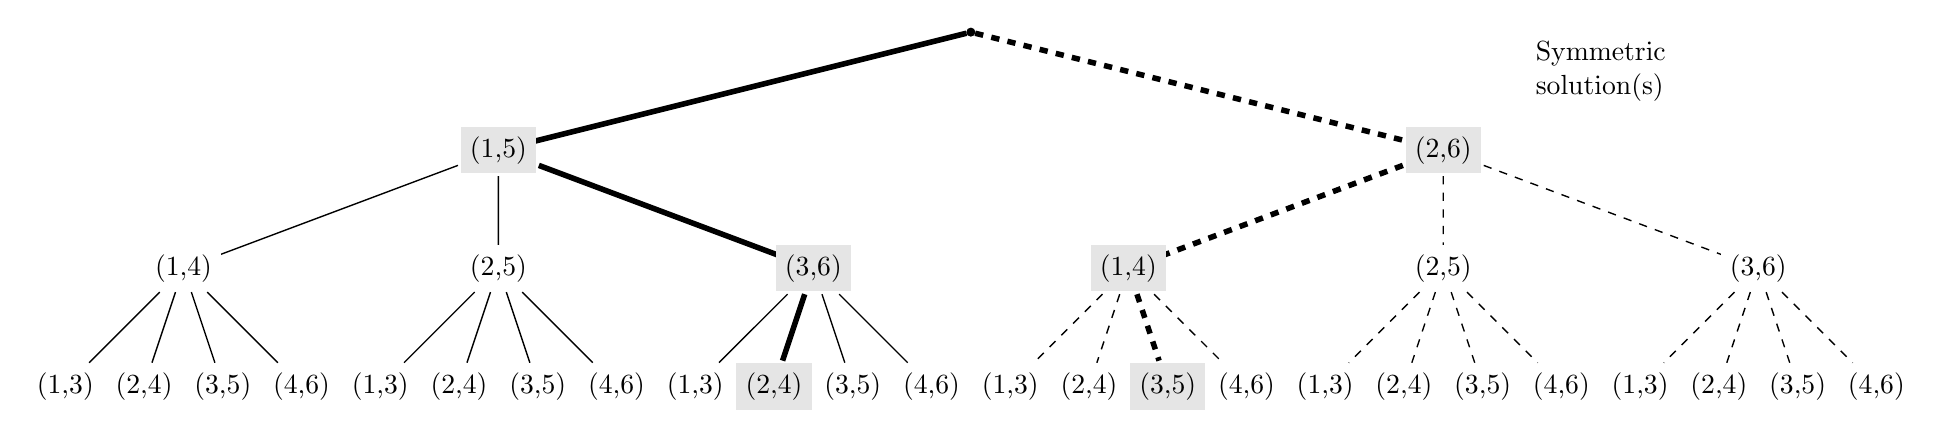
\begin{tikzpicture}[sibling distance=12cm]
%\node at (-13.5,-1.5) {pair 3 positions};
%\node at (-13.5,-3) {pair 2 positions};
%\node at (-13.5,-4.5) {pair 1 positions};
\node [align=left] at (8,-.5) {Symmetric\\solution(s)};
\node  [circle,draw,fill,inner sep=1] {}
  child [line width=2pt] { [sibling distance=4cm] node [fill=black!10] {(1,5)}
    child [line width=.5pt] { [sibling distance=10mm] node [fill=white] {(1,4)}
      child {node {(1,3)}}
      child {node {(2,4)}}
      child {node {(3,5)}}
      child {node {(4,6)}}
    }
    child [line width=.5pt] { [sibling distance=10mm] node [fill=white] {(2,5)}
      child {node {(1,3)}}
      child {node {(2,4)}}
      child {node {(3,5)}}
      child {node {(4,6)}}
    }
    child { [sibling distance=10mm] node [fill=black!10] {(3,6)}
      child [line width=.5pt] {node {(1,3)}}
      child {node [fill=black!10] {(2,4)}}
      child [line width=.5pt] {node {(3,5)}}
      child [line width=.5pt] {node {(4,6)}}
    }
  }
  child [dashed,line width=2pt] { [sibling distance=4cm] node [fill=black!10] {(2,6)}
    child { [sibling distance=10mm] node [fill=black!10] {(1,4)}
      child [line width=.5pt] {node {(1,3)}}
      child [line width=.5pt] {node {(2,4)}}
      child {node [fill=black!10] {(3,5)}}
      child [line width=.5pt] {node {(4,6)}}
    }
    child [line width=.5pt] { [sibling distance=10mm] node [fill=white] {(2,5)}
      child {node {(1,3)}}
      child {node {(2,4)}}
      child {node {(3,5)}}
      child {node {(4,6)}}
    }
    child [line width=.5pt] { [sibling distance=10mm] node [fill=white] {(3,6)}
      child {node {(1,3)}}
      child {node {(2,4)}}
      child {node {(3,5)}}
      child {node {(4,6)}}
    }
  }
;
\end{tikzpicture}
}